\chapter{Problem Domains}
\section{Introduction}
This chapter introduces each of the selected problems. A description of each problem is provided as well as  the grammar used by GE in its attempts to solve the problem is presented in Backus Naur Form. The Santa Fe trail problem consists of an ant searching for food on the Santa Fe Trail, Symbolic Integration and Symbolic Regression attempt to find functions to fit data sets and Blocks is an attempt to stack an ordered set of nine blocks.

\section{Santa Fe Trail}
The Santa Fe Trail is a benchmark problem in Genetic Programming (GP)~\cite{koza}. The objective is to devise a program which can navigate along a 32 X 32 torodial grid picking up pieces of food positioned on the grid. The ant can move left, right, or straight ahead, and can sense food directly in front of it. This ability to sense food is used to select alternate moves to guide the search. For the purpose of this evaluation the ant is allowed 615 time steps, with the exception of sensing food in the square ahead each action consumes one time step. The fitness is the number of pieces of food  (of a possible 88) collected within the 615 time steps. Figure~\ref{trail} shows the trail used in these trials.

Previous research~\cite{langdon} has shown that there is a high density of distinct solutions for this particular problem, with the neighbourhoods of these solutions composed of low fitness programs and a large number of sub-optimal peaks. 
The BNF grammar for this problem is shown below.

\small
\begin{verbatim}
<code>            ::== <line> | <code><line>
<line>            ::== <condition> |  <op> 
<condition>       ::== if(food_ahead()){ <line> else <line>}
<op>              ::== left() | right() | move()
\end{verbatim}
\normalsize



\begin{figure}[]
\centerline{\hbox{
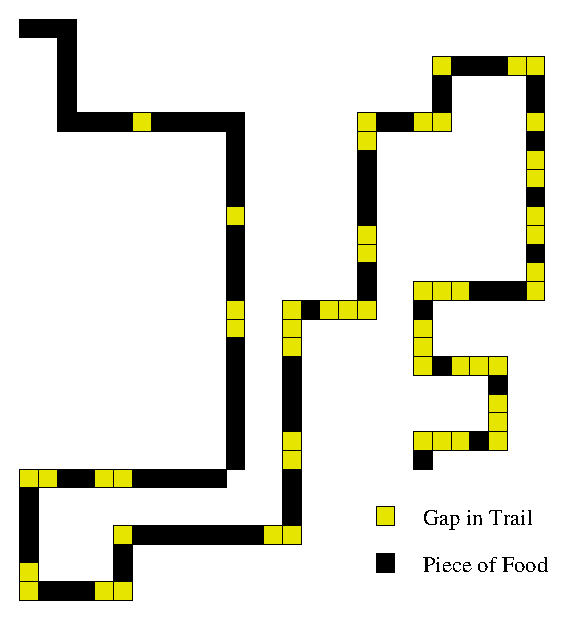
\psfig{file=Chapter4/graphs/trail.ps,width=3in}}}
\caption{\label{trail} Sante Fe Trail.}
\end{figure}



\section{Symbolic Integration}
\label{sym_int_grammar}Symbolic Integration involves finding a function that is the integral of the given curve. The system uses a set of input and output pairs, where the objective is to find the function that maps the inputs to the outputs. For these trials the particular function used was: 

\begin{displaymath}
f(x) = Cos(x) + 2x + 1
\end{displaymath}
with the input values in the range [0...$2\pi$]. The target curve was
\begin{displaymath}
f(x) = Sin(x) + x^2 + x
\end{displaymath}
The fitness for this problem is given by the sum of the absolute value of the difference, taken over 20 fitness cases,  between the individual genetically produced function $f_j(x_i)$ at the domain point $x_i$ and the value of the numerical integral $I(x_i)$. The grammar used is shown below.

\small
\label{sect:symint}\begin{verbatim}
<expr>         :: == <var> | <expr><op><expr> | <pre-op>(<expr>)
                     | (<expr>) 
<var>          :: == X  	                                           
<op>           :: == + | - | / | *                            
<pre-op>       :: == sin | cos | tan | log        

\end{verbatim}
\normalsize

\section{Symbolic Regression}
The objective of the Symbolic Regression problem is to find a function of one independent variable and one dependent variable in symbolic form that fits a sample of 20($x_i,y_i$) data points in the range [-1,+1]. The target function is that used by Koza~\cite{koza}.
\begin{displaymath}
x^4 + x^3 + x^2 + x
\end{displaymath}

The grammar used is identical to that shown for Symbolic Integration.



\section{Block Stacking}
The objective of the block-stacking problem is to produce a specified ordered set of nine blocks stacked as a tower. The starting position involves an initial stack of blocks with the remainder on the table.  Figure~\ref{blocks1} shows a typical starting position.

Three lists are used to specify the problem, the GOAL-LIST specifies the desired final order in which the blocks are to be stacked in the target tower (i.e. "UNIVERSAL"). The STACK-LIST is the ordered set of blocks that are currently in the target tower (where the order is important). The TABLE-LIST is the set of blocks that are currently not in the target tower (where the order is not important). The initial configuration consists of certain blocks in the STACK-LIST and the remaining blocks in the TABLE-LIST. The desired final configuration consists of all the blocks being in the STACK-LIST in the order specified by the GOAL-LIST and no blocks being in the TABLE-LIST.

Three sensors are used to track the system in the formulation of the problem, TB (Top Block) refers to the highest correct block on the stack, NN (Next Needed) is the next block required on the stack as dictated by the specified ordered set of blocks and CS (Current Stack) refers to the top block of the stack. Each of these sensors can assume one of the nine block labels or NIL.  These are illustrated in Figure~\ref{blocks4}. 

\begin{figure}[]
\centerline{\hbox{
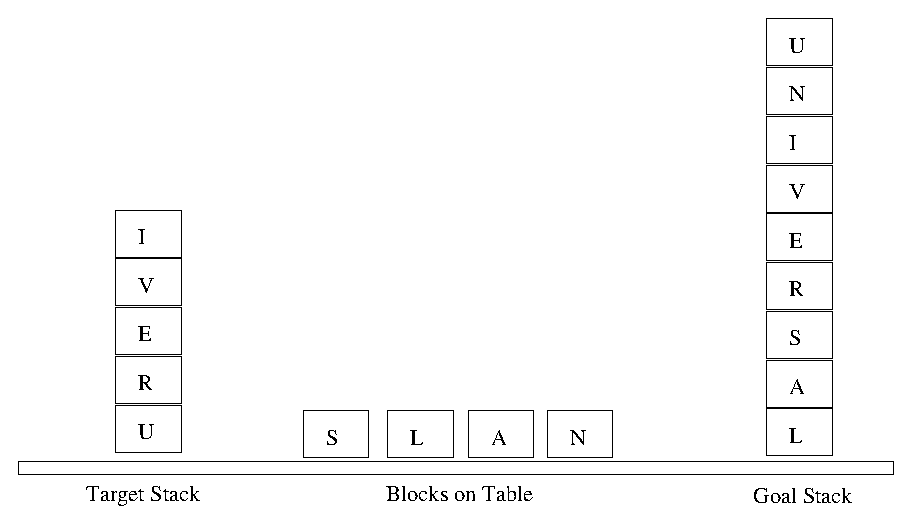
\psfig{file=Chapter4/graphs/blocks1.ps,width=3in}}}
\caption{\label{blocks1} Typical Starting Position for the Blocks Problem.}
\end{figure}

Five functions are available to solve the problem, including NOT (!) and EQUAL (EQ) the usual Boolean negation and equality operators, MS (Move Stack, see Figure~\ref{blocks2} ) moves a single block from the table to the stack. It takes a single argument X  as determined by  one of the three sensors. If X is on the table then X is moved to the top of the stack and MS returns true.
If X is already in the stack, if the table is empty or if X itself is NIL  MS does nothing and returns NIL.  MT (Move Table, see Figure~\ref{blocks3}) moves a block from the top of the stack to the table. It takes a single argument X  as determined by  one of the three sensors. If X is in the stack MT moves the top of the stack to the table and  returns true. 
If X is already on the table, if the table is empty or if X itself is NIL  MT does nothing and returns NIL. 
Finally DU (Do Until) takes two arguments, a body of code that it iteratively executes until the second argument (a predicate) becomes true.

In order to guard against predicates that never evaluate to true an iteration limit is used. This takes the form of 25 iterations for a single DU loop or 100 iterations for all DU operations associated with a particular individual. These limits are those used by Koza~\cite{koza} in his evaluation of the problem using GP. If the DU loop is terminated by the predicate it returns true, termination by the iteration threshold forces the DU loop to return false.
The Grammar associated with this problem is shown below.

\label{blocks_scores}Ten fitness cases are used in this problem. Three of these (the case of the initially correct stack, the empty stack and the empty table) are pre-selected. The other seven are randomly generated. The scores are allocated as follows. Each empty stack is allocated one point, each stack with at least one letter in the correct order is allocated two points, and each fully correct stack is allocated three points. Based on this allocation of points a fully fit individual will score thirty points. 



\begin{figure}[]
\centerline{\hbox{
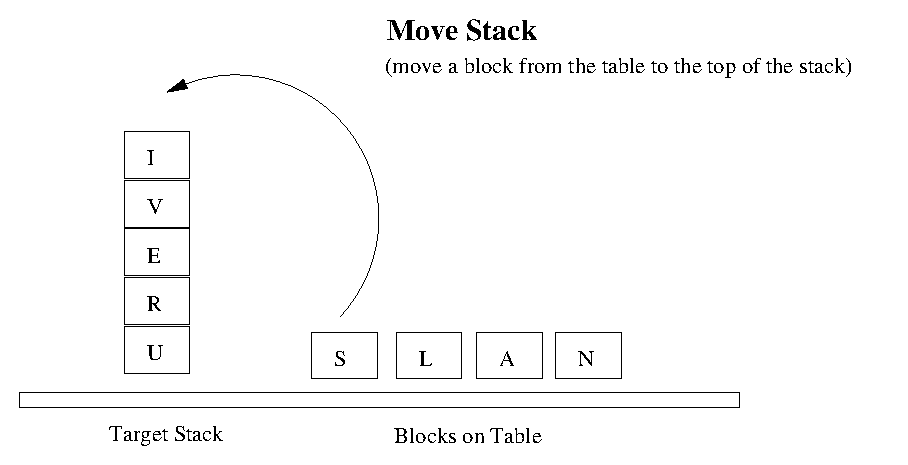
\psfig{file=Chapter4/graphs/blocks2.ps,width=3in}}}
\caption{\label{blocks2} Move Stack operation.}
\end{figure}


\begin{figure}[]
\centerline{\hbox{
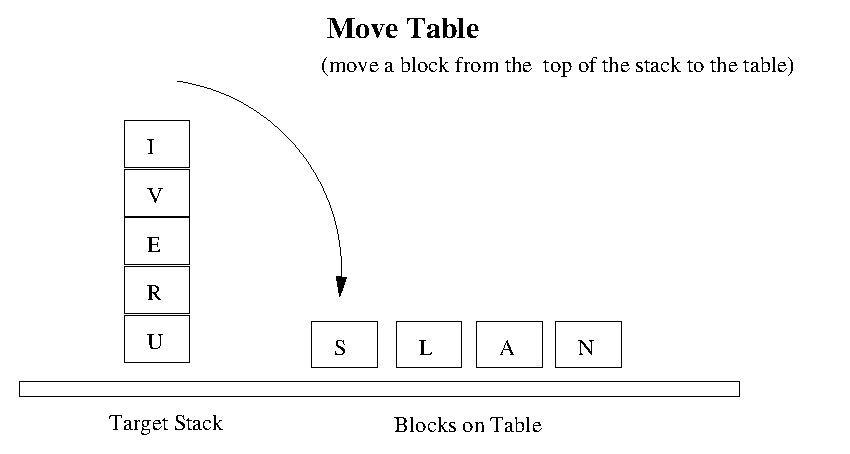
\psfig{file=Chapter4/graphs/blocks3.ps,width=3in}}}
\caption{\label{blocks3} Move Table operation.}
\end{figure}


\begin{figure}[]
\centerline{\hbox{
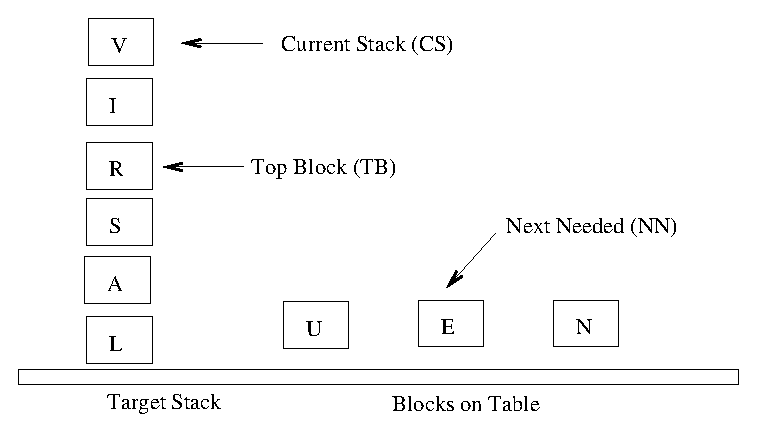
\psfig{file=Chapter4/graphs/blocks4.ps,width=3in}}}
\caption{\label{blocks4} Move Table operation.}
\end{figure}


\small
\begin{verbatim}
<code>            ::== <line> | <code> <line> | <op> <code>  <code>
                      | <pre-op> <code> | <op> <var> <var>
<line>            ::== <control> |  <expr> 
<expr>            ::== MS ( <var> ) | MT ( <var> )s
<control>         ::== DO  <code> UNTIL <code> ODU
<op>              ::== EQ 
<pre-op>          ::== !
<var>             ::== TB | NN | CS
\end{verbatim}
\normalsize


\section{Summary}
In this chapter we have introduced each of the four selected problems, the Santa Fe trail problem, Symbolic Integration, Symbolic regression and Blocks. The problems which are all well-known bench mark problems in the field of Genetic Programming were presented with a brief summary of some of the objectives, characteristics, method for scoring  and a summary in Backus Naur Form of the grammar used by GE to attempt to solve them.























